\documentclass[12pt]{article}

\usepackage[left=0.9in,right=0.9in,top=0.8in,bottom=1.05in]{geometry}
\newcommand{\ligne}[1]{\rule[0.5ex]{\textwidth}{#1}\\}

\usepackage[]{graphicx}
\usepackage{wrapfig}
\usepackage{physics}
\usepackage{color}
\usepackage{amsthm}

\definecolor{coloradoRed}{rgb}{0.80,0.27,0.16}

\usepackage[breakable]{tcolorbox}
\usepackage{graphicx}
\usepackage{enumitem}

\NewDocumentEnvironment{solution}{O{} O{no}}
{
    \begin{tcolorbox}[
        breakable,
        colback=white,
        colframe=black,
        boxrule=0.5pt,
        arc=0pt,
    ]
    \begin{minipage}{\linewidth}

    \textcolor{coloradoRed}{\textbf{Result:}}\par\noindent

    \ifstrequal{#2}{yes}{
        \begin{enumerate}[label=(\alph*)]
            \item 
            \mbox{}\par
    }{}

    \if\relax\detokenize{#1}\relax
        % No image argument -- do nothing
    \else
        
            \centering
            \includegraphics[width=1.0\linewidth]{#1}
       
    \fi

    \ifstrequal{#2}{yes}{
        \end{enumerate}
    }{}

    \end{minipage}
}
{
    \end{tcolorbox}
}
% \newenvironment{proof}
% {\par\noindent\textit{Proof.}}
% {\hfill\qed\par}

\begin{document}

\begin{flushleft}
    \textbf{Department of Applied Mathematics and Statistics} \\
    \textbf{COLORADO SCHOOL OF MINES} \\
    Math $550$: Numerical Solutions of Partial Differential Equations \\
    Charles Girard

\end{flushleft}


\begin{center}
\bf{Numerical PDEs Homework \#0}\\
\bf{Due Tuesday, September 15, 2026}
\end{center}

\vspace{0.3cm}

\noindent \textbf{Problem 1: Finite differences}
Write a matlab code that uses finite differences to compute the first derivative of
$$f(x) = \exp(\sin(x))$$
on the interval $0 \leq x \leq 2\pi$. Use second-order centered differences on internal grid points and first-order one-sided differences at endpoints. 
\begin{enumerate}[label = (\alph*)]
    \item Show a graph of the exact analytic solution $f'(x)$ and your numerical solution $f_n'(x)$. 
    \item Show a relative error convergence plot by plotting the relative error on the y-axis and the grid size $N$ on the x-axis. Measure relative error as 
    $$Err = \frac{\Vert f'(x) - f'_n(x) \Vert_p}{\Vert f'(x) \Vert_p}.$$
    \noindent Plot the error using both the $p=\infty,2$ norms in a log-log scale. The relative errors should be lines with slopes 1 and 3/2 respectively, i.e. it scales with $\displaystyle \frac{1}{N}, \frac{1}{N^{3/2}}$. Extra Credit: The $3/2$ slope is strange, why is that happening?
\end{enumerate}

\begin{solution}
    \begin{enumerate}[label=(\alph*)]
        \item
        \begin{minipage}[t]{\linewidth}
            \mbox{}\par
            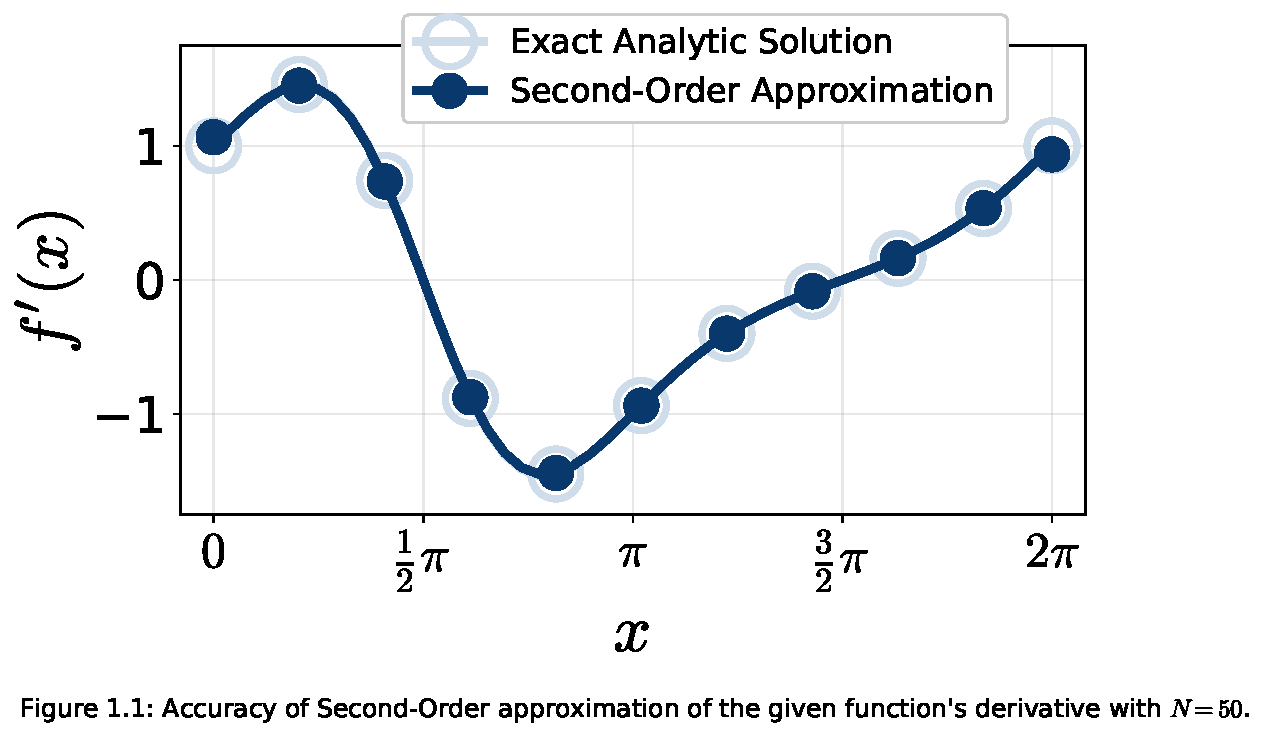
\includegraphics[width=1.0\linewidth]{figs/figure_1_1.pdf}
        \end{minipage}
        \item
        \begin{minipage}[t]{\linewidth}
            \mbox{}\par
            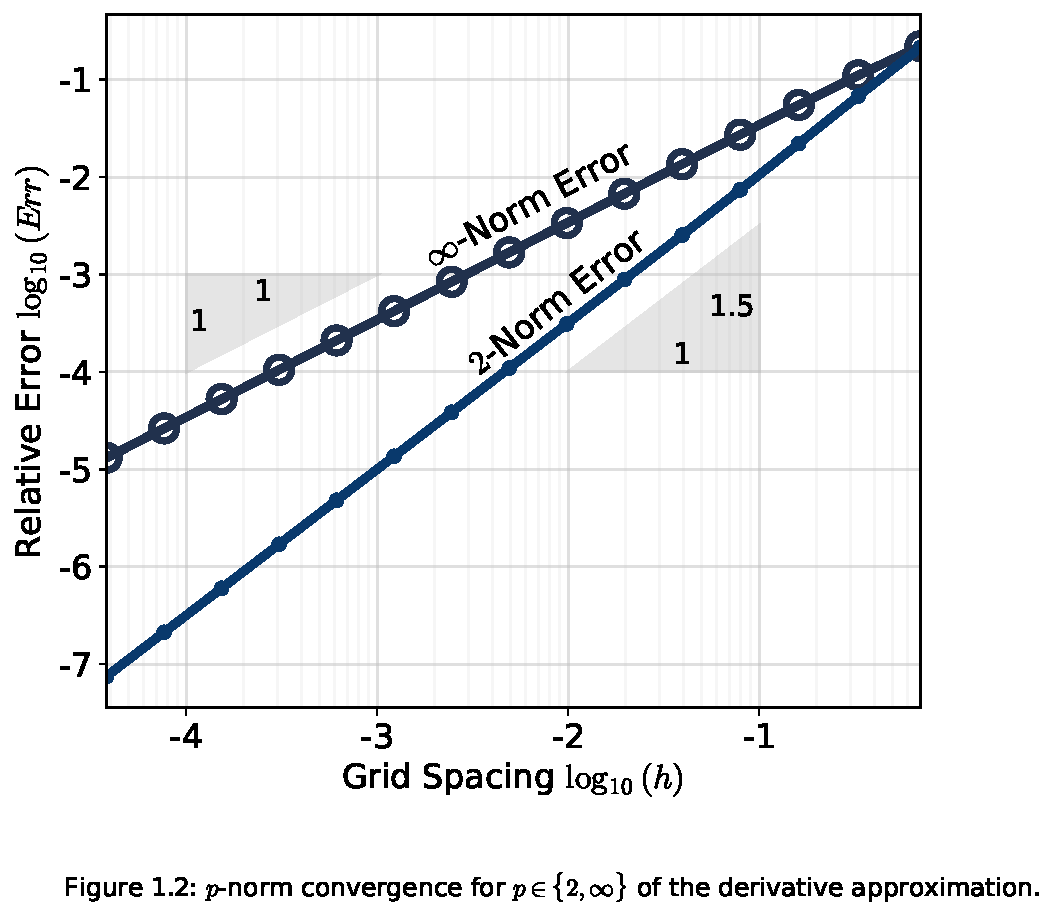
\includegraphics[width=1.0\linewidth]{figs/figure_1_2.pdf}
        \end{minipage}
            \begin{proof}
            We begin with the given equation for the $2$-norm error:

            \[
                Err_2 = \frac{\lVert f'(x) - f_n'(x)\rVert_2}{\lVert f'(x) \rVert_2}
            \]

            When order notation is introduced, the $3/2$ slope property appears.
            To begin, state that for all $x_i$, its derivative does not depend on $h$:
            \[
                f'(x_i) \to O(1), \quad i \in \{1,2,\dots,N\}
            \]
            Next, consider the error of the first-order-evaluated endpoints, for which it is well known their error scales with $h$:
            \[
                \lvert f'(x_i) - f_n'(x_i) \lvert \to O(h), \quad i=1,N
            \]
            Similarly, the error for the second-order-evaluated interior points:
            \[
                \lvert f'(x_i) - f_n'(x_i) \lvert \to O(h^2), \quad i \in \{2,3,\dots,N-1\}
            \]
            Therefore the $2$-norm of the error at $x_i$ and the analytic solution at $x_i$ can be calculated:
            \[
                \lVert f'(x) - f_n'(x)\rVert_2 = \left( \sum_{i=1}^{N} f'(x_i) - f_n'(x_i)^2 \right)^{1/2} \\
                \to \sqrt{O(h)^2 + O(N) \cdot  O(h^2)^2},
            \]
            where $O(h)$ comes from the two endpoints' error. Following simplifications:
            \[  \begin{aligned}
                O(h)^2 = O(h^2),\\
                O(N) \cdot O(h^2)^2 = O(h^3) \quad (\text{by } N \to O(1/h)),\\
                O(h^2) + O(h^3) = O(h^2) \quad (\text{by }h\text{ small}),\\
                \sqrt{O(h^2)} = O(h)
            \end{aligned} \]
            the order of the numerator term (that is, the norm of the error at every $x_i$) is yielded:
            \[
                \lVert f'(x) - f_n'(x)\rVert_2 \to O(h)
            \]
            A similar and more straightford process occurs for the denominator term (that is, the norm of the analytic solution at every $x_i$):
            \[
                \lVert f'(x) \rVert_2 = \left( \sum_{i=1}^N f'(x_i) \right)^{1/2} \\
                \to \sqrt{O(N)} \\
                = O(h^{-1/2})
            \]
            Therefore the order for the convergence emerges:
            \[
                Err_2 \to \frac{O(h)}{O(h^{-1/2})} = O(h^{3/2}) = O(\frac{1}{N^{3/2}})
            \]
            \end{proof}
    \end{enumerate}
\end{solution}

\vspace{0.5cm}

\noindent \textbf{Problem 2: Second-order derivatives}
Repeat problem 1 but compute the second derivative $f''(x)$. Assume periodicity and wrap around the grid instead of using one-sided finite differences.

\begin{solution}[figs/figure_2_1.pdf]
    \begin{center}
    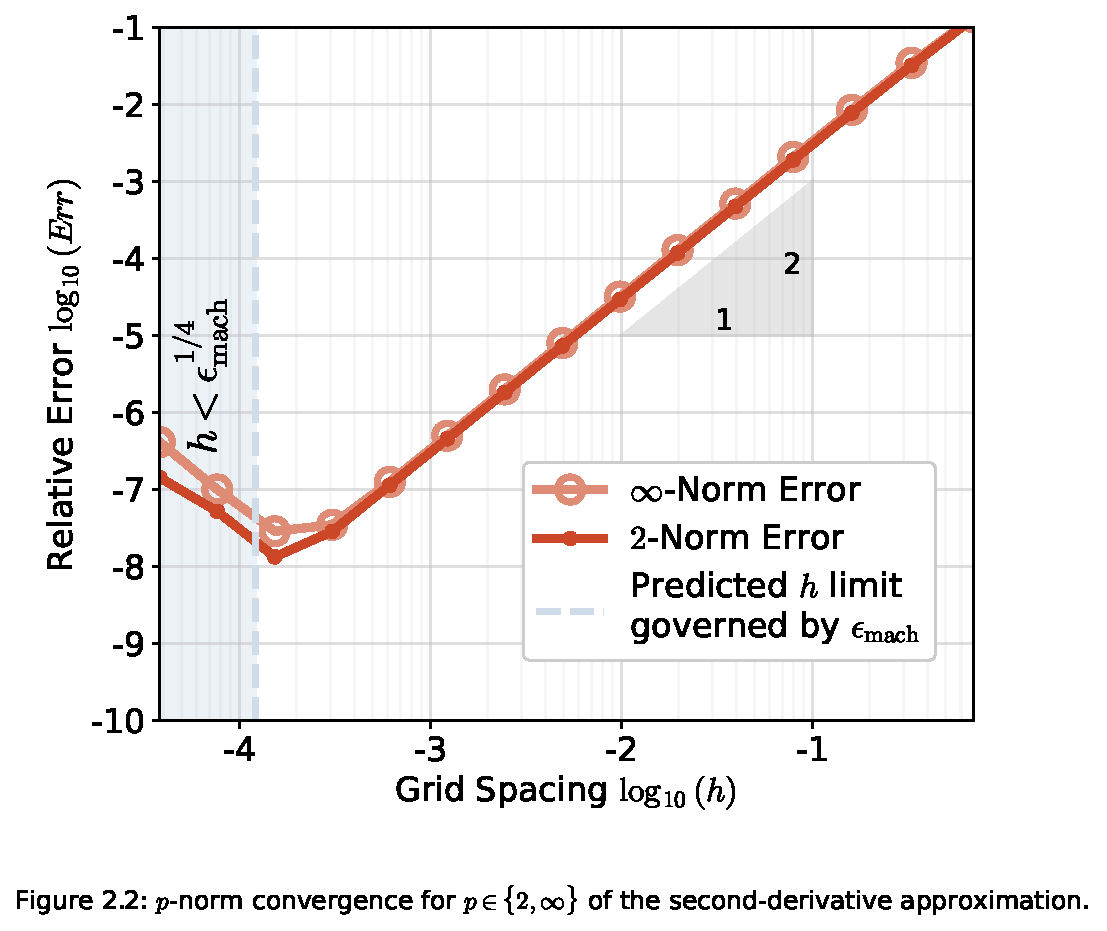
\includegraphics[width=1.0\linewidth]{figs/figure_2_2.pdf}
    \end{center}
\end{solution}

\vspace{0.5cm}

\noindent \textbf{Problem 3: ODE}
Consider the ODE
$$\dv[2]{u}{x} + \sin(x) \dv{u}{x} + u(x) = f(x)$$
defined on $0 \leq x \leq 5$. Solve the ODE using second-order finite difference methods with the Dirichlet conditions. Use $u(x) = \sin(x)$ to test your solution by finding boundary conditions and the necessary forcing function $f(x)$. Show an error plot that proves your method converges with second order. 

\begin{solution}[figs/figure_3_1.pdf]
    \begin{center}
    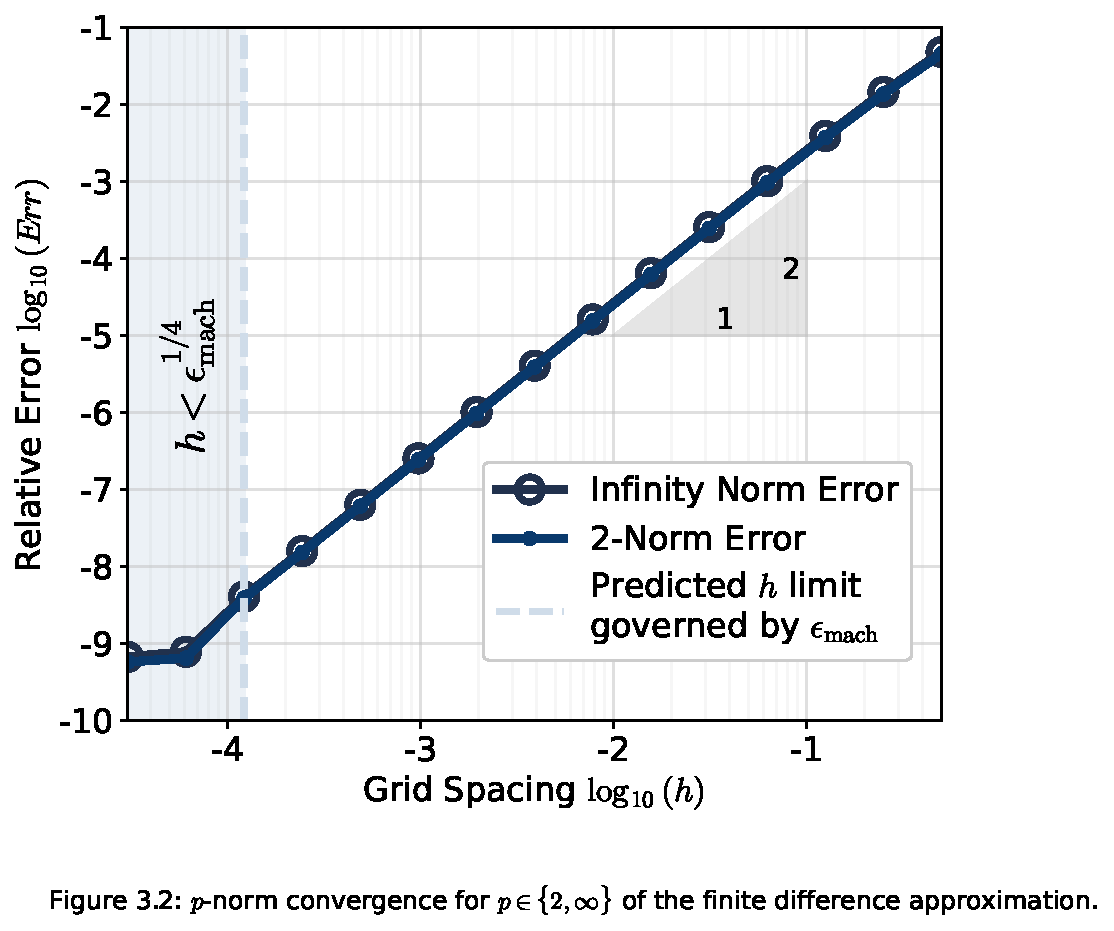
\includegraphics[width=0.8\linewidth]{figs/figure_3_2.pdf}
    \end{center}
\end{solution}

\vspace{0.5cm}
\noindent \textbf{Problem 4: Poisson Equation}
Use finite difference methods to solve the Poisson equation $\nabla^2 u = f(x,y)$ in the domain $x \in [0, 5], y \in [0, 5]$. Use the test solution $u(x,y) = \sin(x)\cos(y)$. 

\begin{enumerate}[label=(\alph*)]
    \item Apply Dirichlet conditions on all boundaries so that $u(x,y)$ satisfies the PDE and the boundary conditions, and show a plot of your solution and a second order convergence plot (similar to the first three problems). 
    \item Modify your code to apply Neumann conditions on all boundaries. \textbf{This won't work.} Why not? -- both in terms of the linear algebra and in terms of the actual PDE we want to solve. Suggest a solution to the issue.
\end{enumerate}

\begin{solution}[figs/figure_4_1.pdf][yes]
    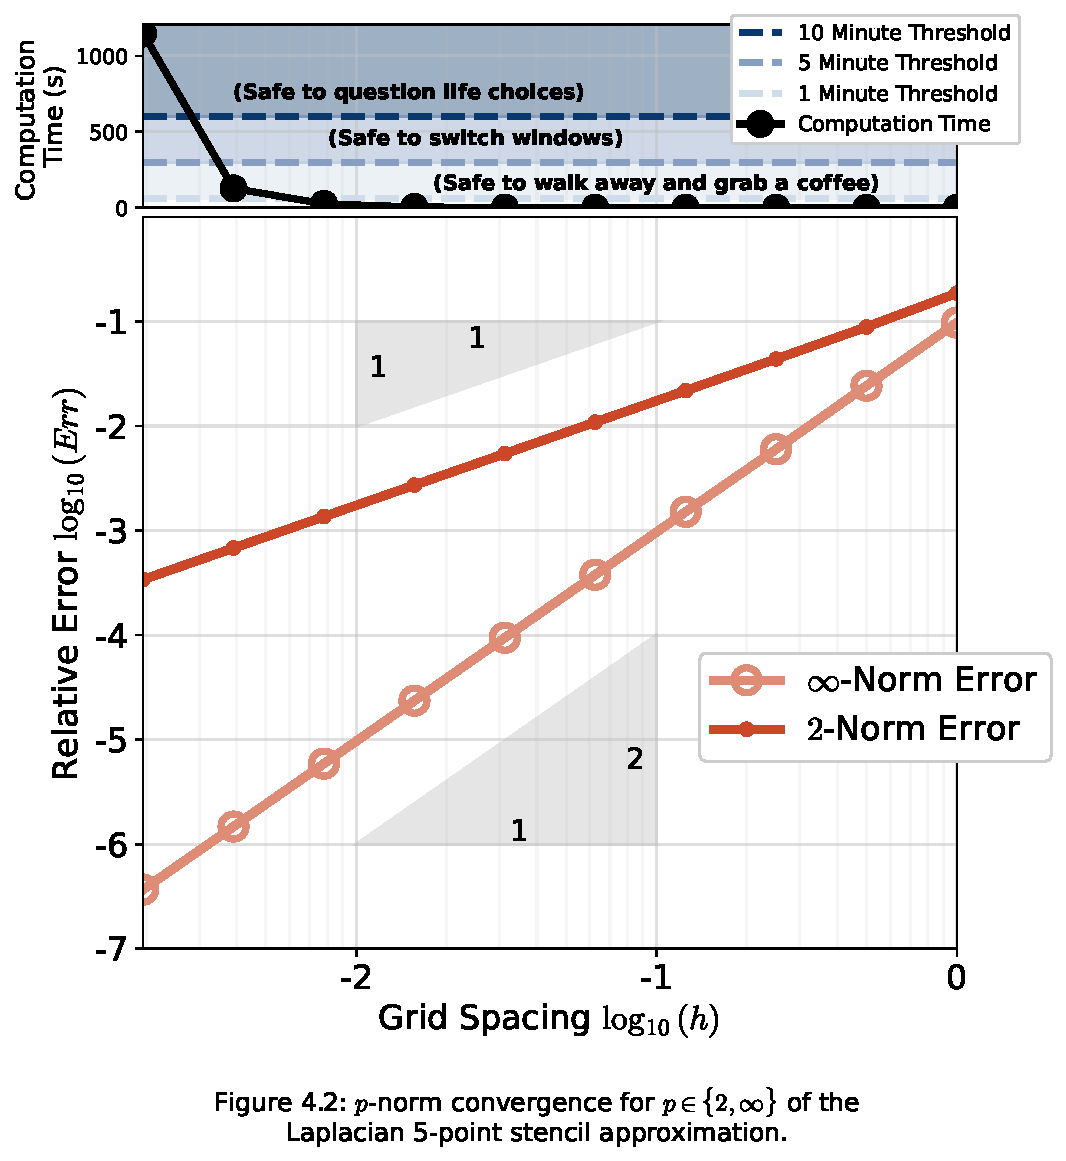
\includegraphics[width=1.0\linewidth]{figs/figure_4_2.pdf}
    \begin{enumerate}[label=(\alph*), start=2]
        % \setcounter{enumi}{1}
        \item \begin{proof}
        Explanation of why Neumann fails:

        The governing equations are only concerned with the first and second derivatives of $u$. 

        The fundamental theorem of calculus reminds us that integrating an undefined function gets us an arbitrary constant:

        $$
            \int g(x)\,dx = \int g(x)\,dx\,+C
        $$

        That tells us:

        $$
            u \text{ solves some property based on } u_x,\,u_y \implies u+C \text{ solves the same property.}
        $$

        Therefore, the linear equation for $u_{i,j}$ is *underdetermined* and will be correct, +/- a constant, $C$. Which, based on the solver used, can be close to the maximum magnitude the machine can compute.
        \end{proof}
        It can be, for example,  accurate to give or take a constant of \textbf{2.3 100 billions.}
        \vspace{0.5cm}\mbox{}\par
        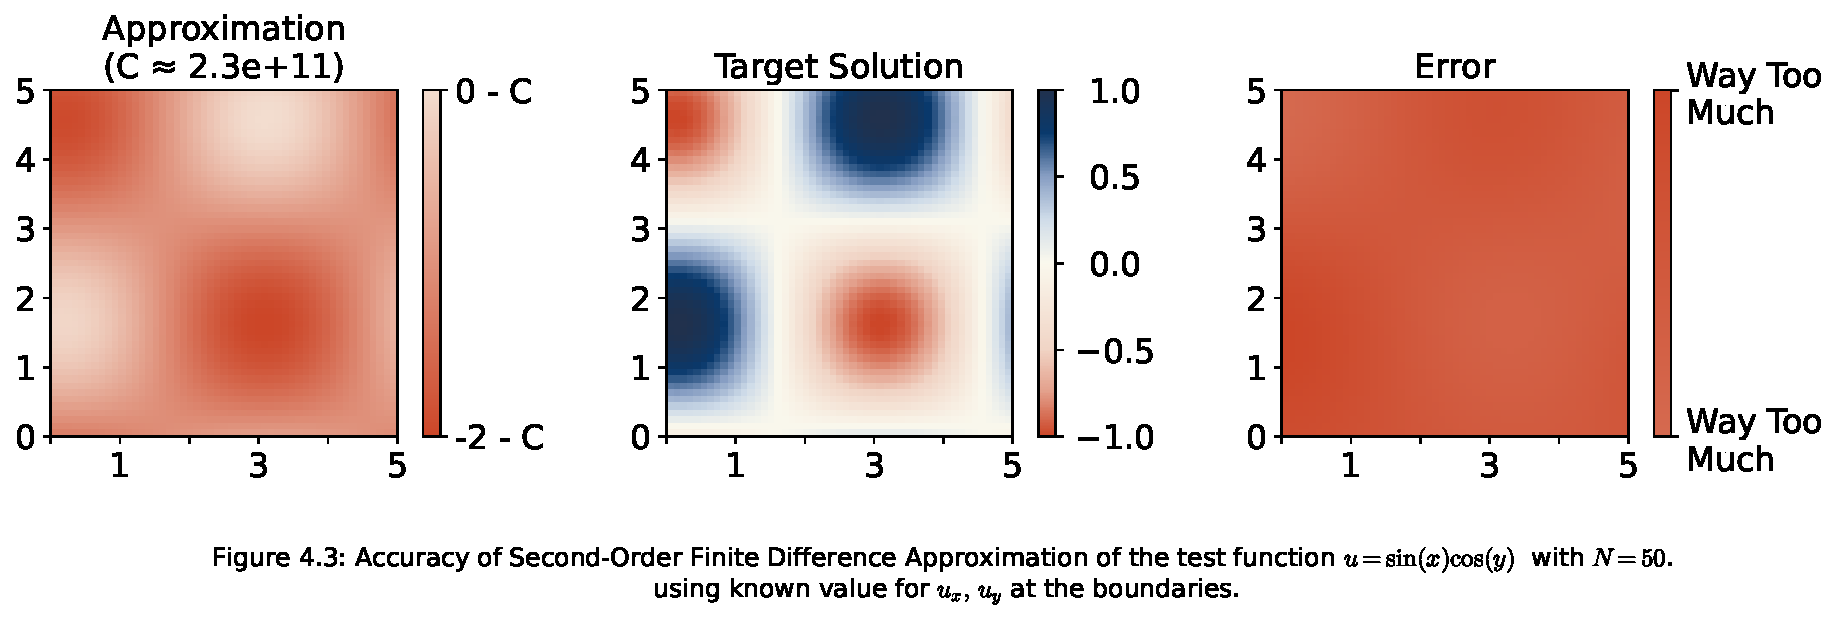
\includegraphics[width=1.0\linewidth]{figs/figure_4_3.pdf}
        \vspace{0.5cm}\mbox{}\par
        However, let's say we know that this solution is correct to a constant, albeit a large one. If we also know what the minimum of the functin \textit{should} be, then we can adjust accordingly:
        \vspace{0.5cm}\mbox{}\par
        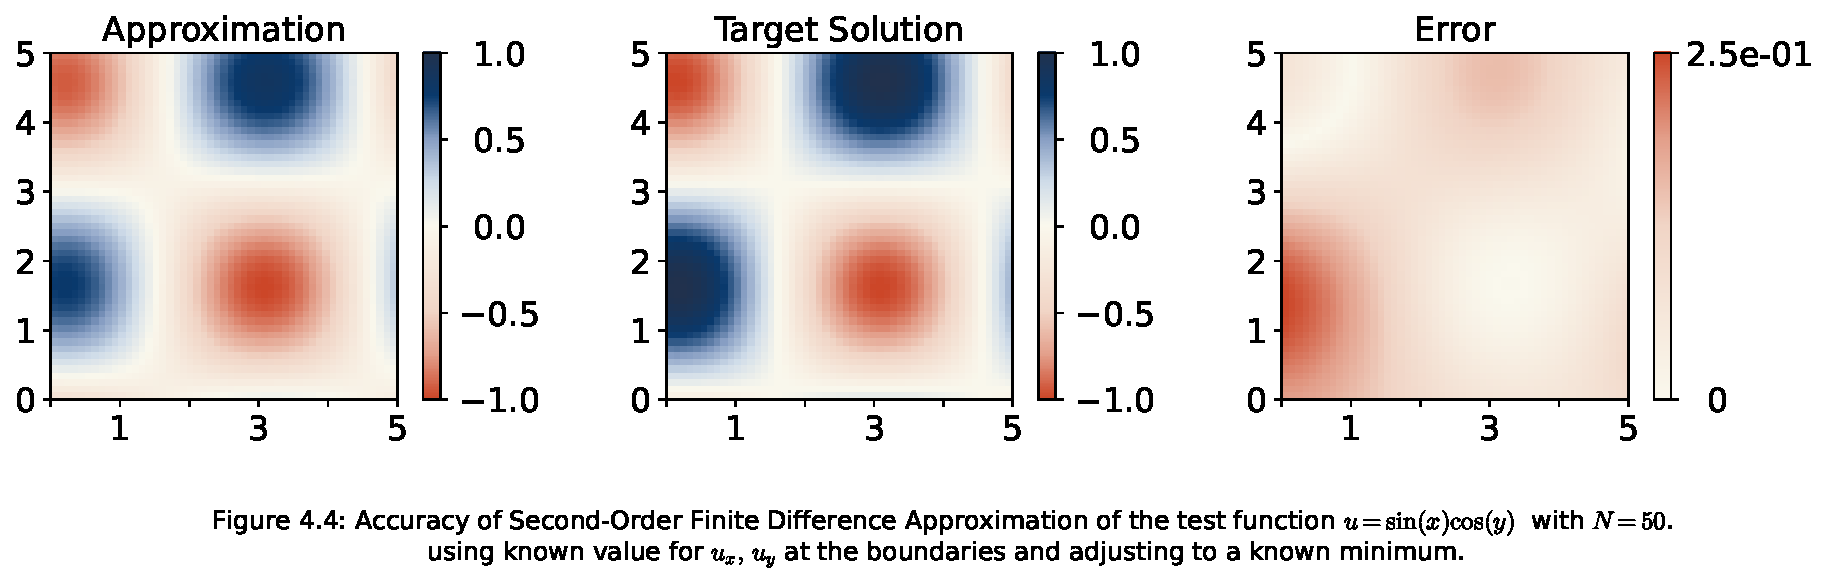
\includegraphics[width=1.0\linewidth]{figs/figure_4_4.pdf}
        \vspace{0.5cm}\mbox{}\par
        Alternatively, if we know a property like oscellacion about zero, we can enforce that the boundary's norm is zero (that is, $u(x,y)$ sums to zero on the boundary):
        \vspace{0.5cm}\mbox{}\par
        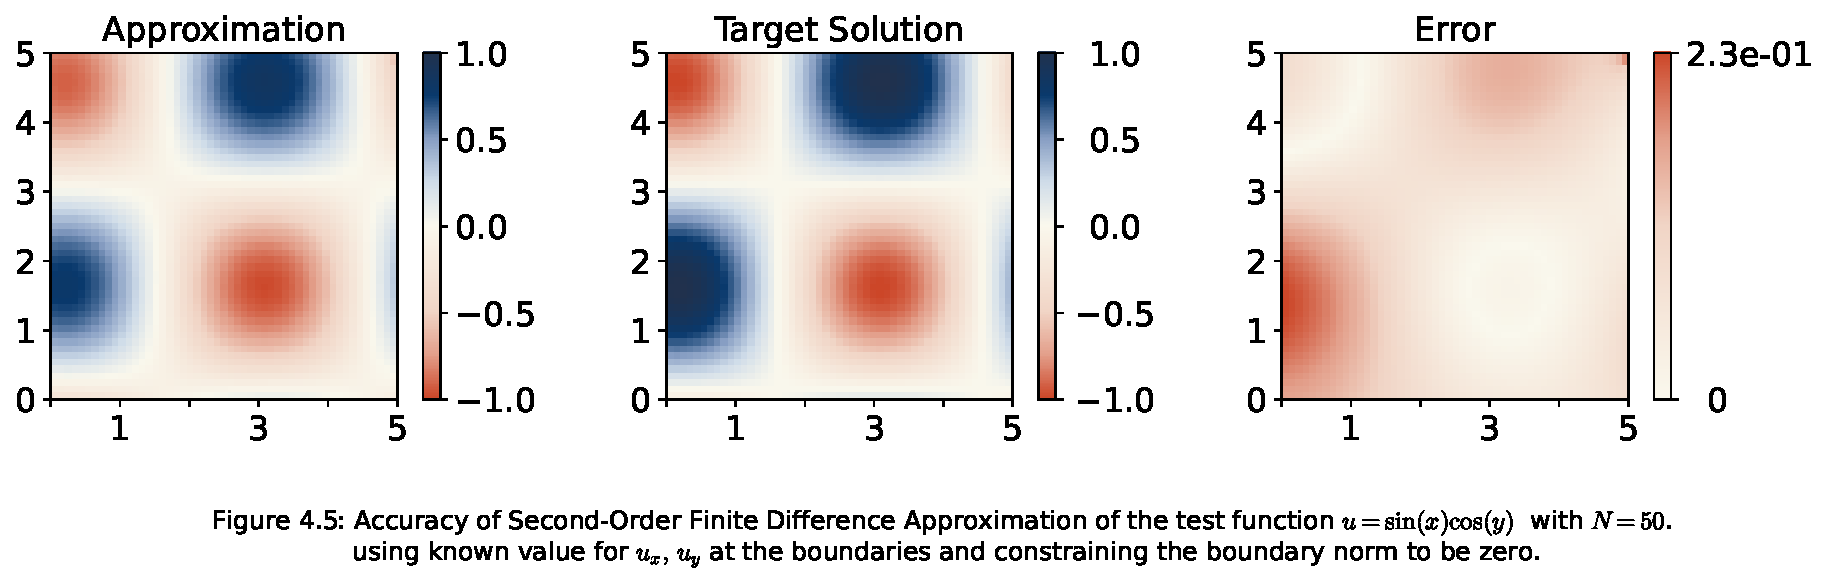
\includegraphics[width=1.0\linewidth]{figs/figure_4_5.pdf}
    \end{enumerate}
\end{solution}

\end{document}